\documentclass[final,12pt,report]{jsbook}
\usepackage{mymacros}
\usepackage{mymacro}
\usepackage{okumacro}
\newcommand{\dmp}[1]{\fixme{\texttt{<<}柳澤に相談\texttt{>>} #1}}

\makeatletter
\def\@pdfm@dest#1{%
  \Hy@SaveLastskip
  \@pdfm@mark{dest (#1) [@thispage /\@pdfview\space @xpos @ypos null]}%
  \Hy@RestoreLastskip
}
\makeatother
\pagestyle{empty}

\title{
{\LARGE\sffamily\gtfamily
O\ \ J\ \ L\ \ 報\ \ 告\ \ 書\\
}
\vspace*{.6in}
{\huge\sffamily\gtfamily
トレースログ可視化ツール(TLV)に対する\\
機能追加とリファクタリング\\
}
\vfill\vfill\vfill
}
\author{
\LARGE\sffamily\gtfamily
350802246\ \ \ \ 水野 洋樹\\
}
\date{
\vfill
\Large\sffamily\gtfamily
名古屋大学 大学院情報科学研究科\\[.2in]
情報システム学専攻\\[.2in]
2010年1月
\vfill
}
\renewcommand{\baselinestretch}{1}
\begin{document}
\pagestyle{empty}
%%%%%%%%%%%%%%%%%%%%%%%%%%%%%%%%%%%%%%%%%%%%%%%%%%%%%%%%%%%%%%%%%%%%%%%%%%
% 和文要旨
%-------------------------------------------------------------------------
\vspace*{-1in}
\begin{center}
\Large\sffamily\gtfamily
トレースログ可視化ツール(TLV)に対する\\
機能追加とリファクタリング
\end{center}
\begin{flushright}
\large\sffamily\gtfamily
350802246\ \ \ \ 水野 洋樹
\end{flushright}
\begin{center}
\large\sffamily\gtfamily 要旨
\end{center}

近年、組込みシステムの分野においてもマルチコアの導入が進んでいる.
マルチコア環境では、各コアが独立し
て並列に動作するため、ブレークポイントやステップ実行を用いた実行時のデ
バッグが困難である.そのため、 RTOS等のトレースログを用いた
デバッグが有用と考えられるが、サイズの大きなトレースログを直接開
発者が扱うのは困難である。そこ
で本OJLでは、トレースログを可視化表示することで解析を容易にし、マルチコ
ア環境でのアプリケーション開発を支援である
\textbf{TraceLogVisualizer(TLV)}の開発を目的とする。

TLVは,各種RTOSやシミュレータ,エミュレータなどが出力するトレースログを
可視化表示するツールである. TLVは,トレースログを変換ルールに従い標準形式トレースログに変換し,
標準形式トレースログに対して可視化ルールを適用し、図形データの生成を行う.
TLVでは,変換ルールと可視化ルールを外部ファイルとして与えることで,汎用
性と拡張性を実現する.

本OJLはフェーズに分割して開発を行なった.
フェーズの終了ごとにTLVのリリースを行ない、要求の収集を行なった。

%% 2008
%% 年度後期のフェーズ3では単体テスト・システムテストと,機能拡張のための要
%% 件抽出を行った.2009年度前期のフェーズ4では要求の収集を行い、スクリプト
%% 拡張機能を実装した。2009年度後期のフェーズ5ではアプリケーションの動作速
%% 度向上を目的として、リファクタリングを行なった。また、フェーズ4の内容を
%% 反映させたバージョン1.1を公開した。

リリースを通じて要求を収集したところ、(1)従来の変換ルール,可視化ルールでは行なえない
複雑な可視化を行いたい、(2)トレースログの解析が遅いため高速化して欲しい、という要求が強かった。

(1)の複雑な可視化を実現するために、
\MARU{1}変換ルールと可視化ルールを拡張する
\MARU{2}変換用の言語を開発する
\MARU{3}外部プロセスで変換・図形生成を行なえるようにする、
の3つの方針を比較検討した。
実装コストを利用者の学習コストを考慮し、\MARU{3}の方法を選択し、
変換と図形生成を外部のプロセスで行なえるよう
にするスクリプト拡張機能を実装した。外部プロセスは任意のプログラミング
言語で記述できるため、複雑な可視化を行なえる。

%(1)変換ルールと可視化ルールを拡張する
%(2)変換用の言語を開発する
%(3)外部プロセスで変換・図形生成を行なえるようにする、
%の3つの方針を比較検討した。

%% (1)の方法はルールが複雑化しているため実装コストが大きい。
%% (2)の方法も新たな言語の設計が必要であるため実装コストが大きい。
%% また利用者が新たな言語を学習する必要がある。
%% そこで、実装コストを利用者の学習コストを考慮し、(3)の方法を選択した。

%% スクリプト拡張を行なった後のTLVの変換プロセスを図\ref{fig:se}に示す。外
%% 部プロセスは任意のプログラミング言語で記述できるため、複雑な可視化を行
%% なえる。外部プロセスとは、標準入出力によって通信が行なわれる。

%% スクリプト拡張によって、CPU利用率の可視化を行なった例を図\ref{fig:cpu}に示す。

%% \begin{figure}[b]
%% \begin{minipage}{0.45\columnwidth}
%% \centering
%% \includegraphics[width=\textwidth]{se.eps}
%% \caption{外部プロセスによる変換・図形データの生成の実現}\label{fig:se}
%% \end{minipage}
%% \begin{minipage}{0.45\columnwidth}
%% \centering
%% 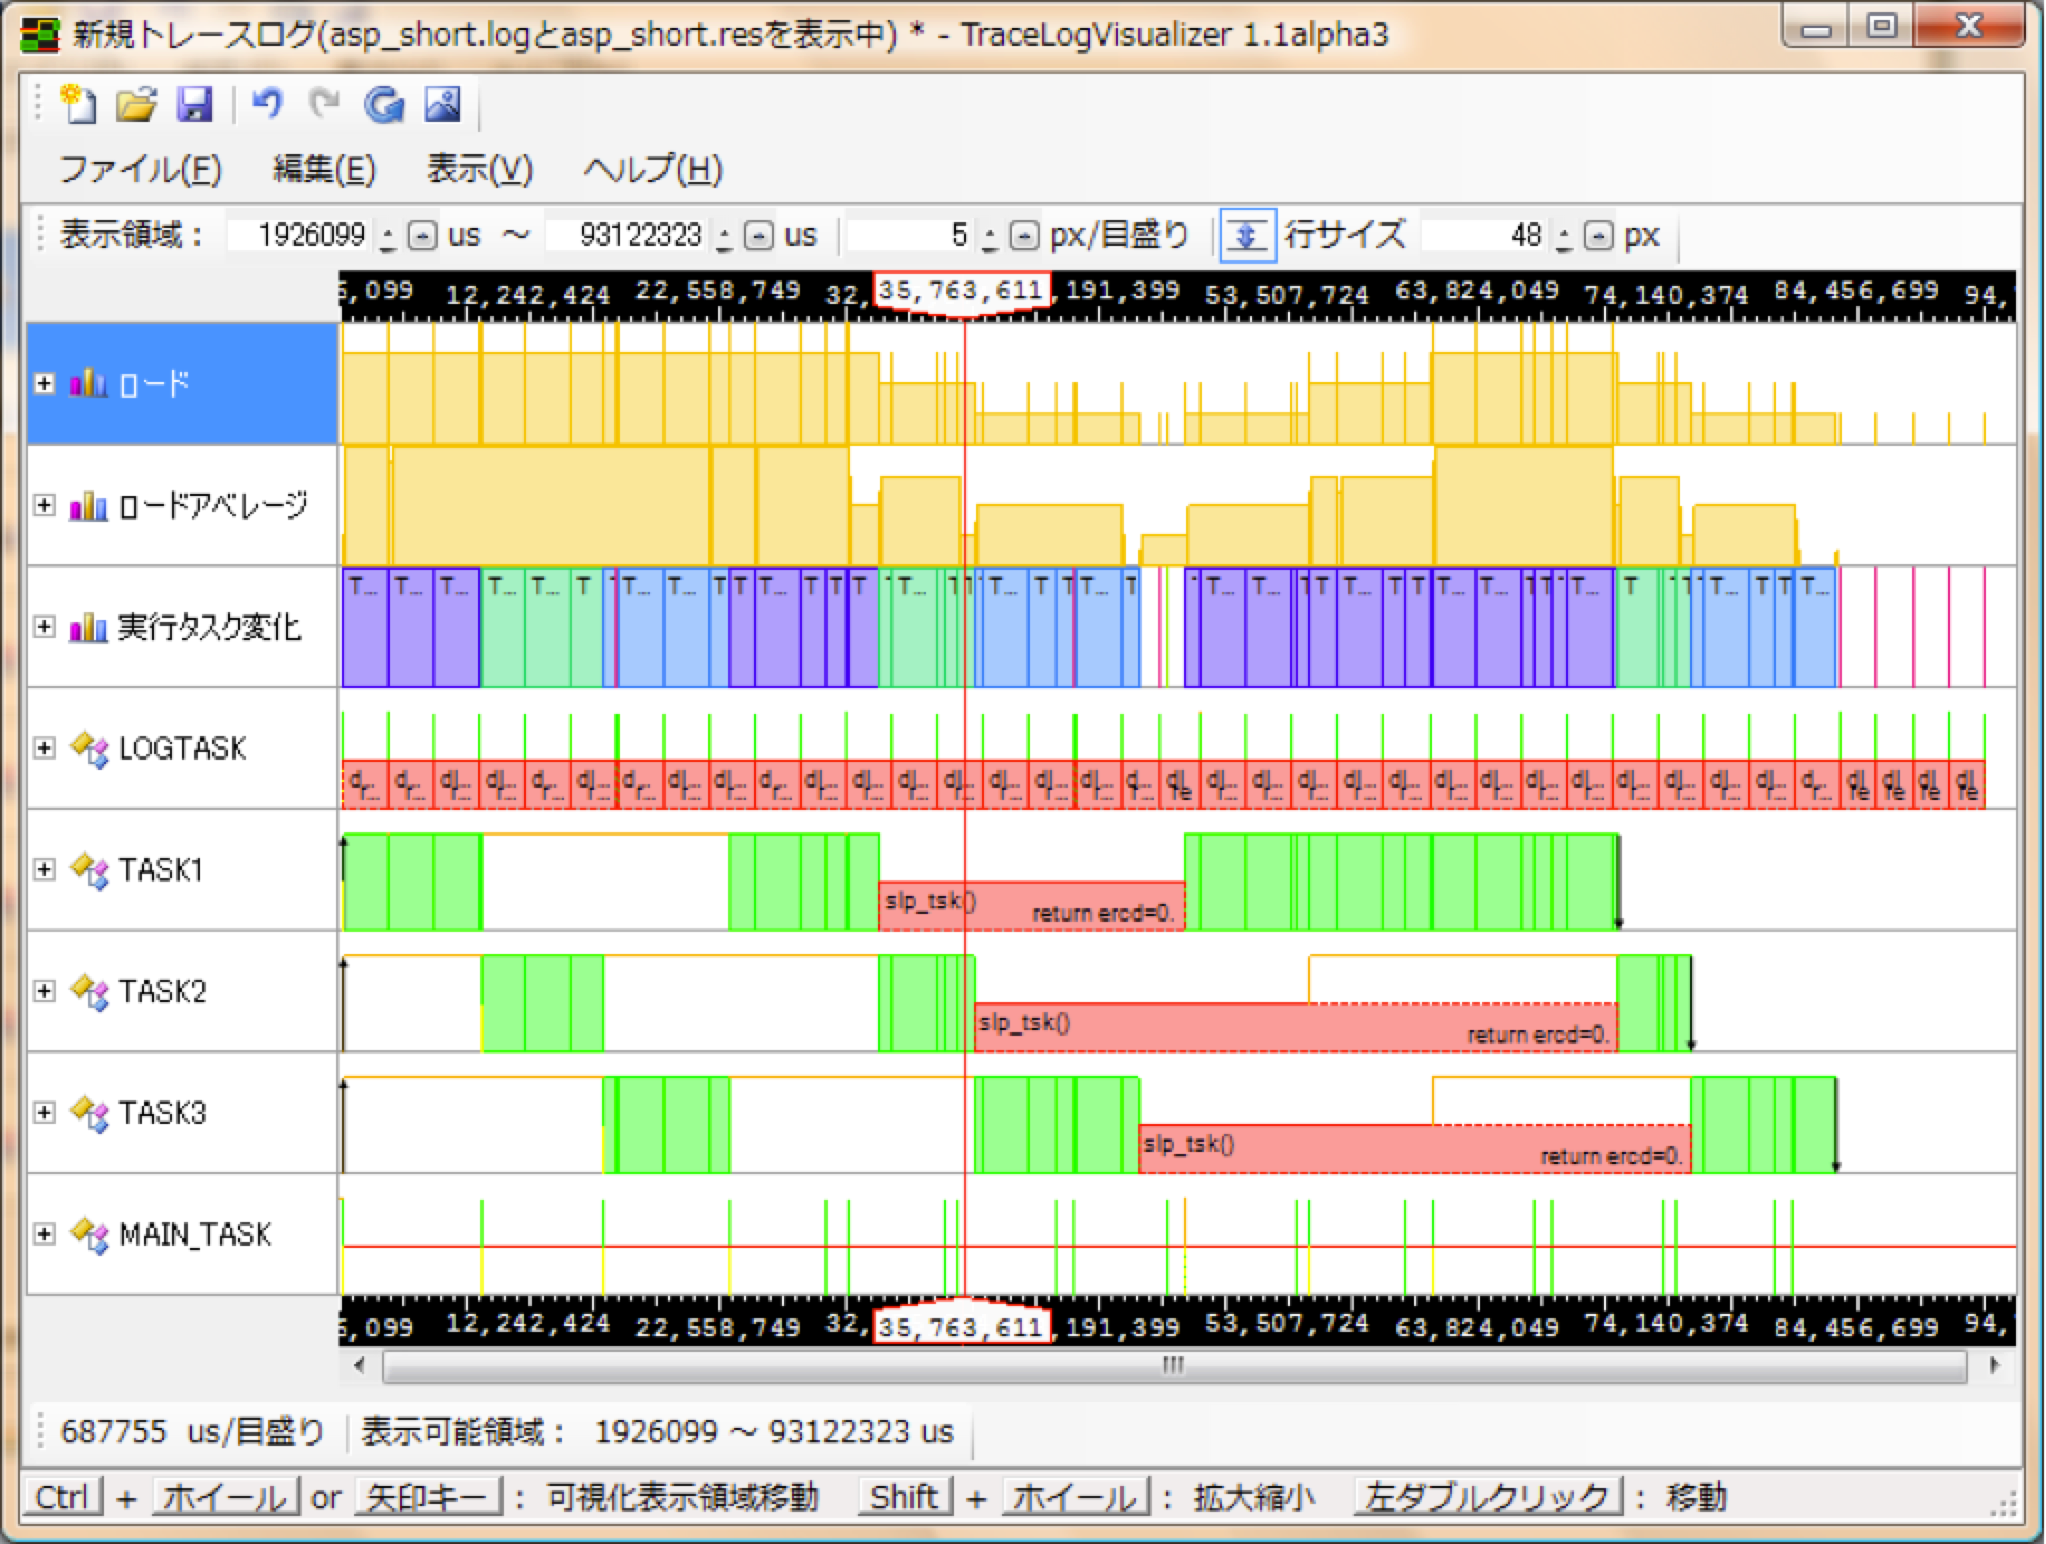
\includegraphics[width=0.8\textwidth]{cpu.png}
%% \caption{CPU利用率の可視化}\label{fig:cpu}
%% \end{minipage}
%% \end{figure}

(2)の変換の高速化の行なうにあたり、トレースログへの変換に関するソースコー
ドが複雑化している点が障害となった。そこで,関連するソースコードの調査
した。
調査の結果、クラス設計に大きな問題はなかったが、
多くのクラスにおいて、複雑な処理を行なうメソッドが存在しており、これが
ソースコードを複雑化さている原因であった。
そこで、複雑化したメソッドの整理をリファクタリングの目的とした。

\newpage

\maketitle
%%%%%%%%%%%%%%%%%%%%%%%%%%%%%%%%%%%%%%%%%%%%%%%%%%%%%%%%%%%%%%%%%%%%%%%%%%
\pagestyle{plain} \pagenumbering{roman}
\setcounter{page}{1}
\setcounter{tocdepth}{2}
\tableofcontents

\clearpage
%%%%%%%%%%%%%%%%%%%%%%%%%%%%%%%%%%%%%%%%%%%%%%%%%%%%%%%%%%%%%%%%%%%%%%%%%%
% 本文
%-------------------------------------------------------------------------
\pagestyle{plain} \pagenumbering{arabic}
\setcounter{page}{1}

\input{intro.pat.tex}
\input{tlv.pat.tex}
\input{actual.pat.tex}
\input{se.pat.tex}
\input{ref.pat.tex}
\input{conclusion.pat.tex}

\chapter*{謝辞}
TLVを開発するにあたり,ご指導を頂きました名古屋大学大学院情報科学研究科
情報システム学専攻組込みリアルタイムシステム研究室の高田広章教授
に深く感謝致します.
また、開発プロジェクトマネージャとして
日頃より多くのご助言を頂きました
愛知県立大学情報科学部情報システム学科の山本晋一郎准教授、
名古屋大学大学院情報科学研究科情報システム学専攻組込みリアルタイムシステム研究室の
本田晋也助教、
企業出身者としての立場から実践的なご意見を頂きました同研究科付属組込みリアルタイム研究センターの長尾卓哉研究員
に深く感謝致します.

\begin{thebibliography}{99}%\addcontentlzissekiline{toc}{chapter}{\bibname}
\bibitem{goto} 後藤隼弐 『OJLによるトレースログ可視化ツールの開発』修士論文,名古屋大学,2009

\bibitem{ipsj}
後藤隼弐,
本田晋也,
長尾卓哉,
高田広章『トレースログ可視化ツールの開発』
情報処理学会 第 139 回 システムLSI設計技術(SLDM)研究会, 2009年 2月 26日

\bibitem{fuzzing}
Michael Sutton, Adam Greene, Pedram Amini, 園田道夫,伊藤裕之
『ファジング:ブルートフォースによる脆弱性発見手法』
毎日コミュニケーションズ, 2008年5月28日

\bibitem{PARTNER-JET}
JTAG ICE PARTNER-Jet,http://www.kmckk.co.jp/jet/,最終アクセス2009年1月14日

\bibitem{watchpoint}
WatchPointデバッガ,https://www.sophia-systems.co.jp/ice/products/watchpoint,最終アクセス2009年1月14日

\bibitem{QNXMomentics}
QNX Momentics Tool Suite,http://www.qnx.co.jp/products/tools/,最終アクセス2009年1月14日

\bibitem{eBinder}
eBinder,http://www.esol.co.jp/embedded/ebinder.html,最終アクセス2009年1月14日

\bibitem{LKST}
LKST(Linux Kernel State Tracer) - A tool that records
traces of kernel state transition as events,http://oss.hitachi.co.jp/sdl/english/lkst.html,最終アクセス2009年1月14日

\bibitem{SystemTap}
Prasad, V., Cohen, W., Eigler, F. C., Hunt, M., Keniston, J. and Chen, B.: Locating system problems using dynamic instrumentation. Proc. of the Linux Symposium, Vol.2, pp.49–64, 2005.

\bibitem{LTTng}
Mathieu Desnoyers and Michel Dagenais.: The lttng tracer : A low impact performance and behavior monitor for gnu/linux. In OLS (Ottawa Linux Symposium) 2006, pp.209–224, 2006.

\bibitem{Dtrace}
R. McDougall, J. Mauro, and B. Gregg.: Solaris(TM) Performance and Tools: DTrace and MDB Techniques for Solaris 10 and OpenSolaris. Pearson Professional, 2006.

\bibitem{LTTV}
Mathieu Desnoyers and Michel Dagenais.: OS Tracing for Hardware, Driver and Binary Reverse Engineering in Linux. CodeBreakers Journal Article, vol.4, no.1, 2007.

\bibitem{Chime}
OpenSolaris Project: Chime Visualization Tool for DTrace,http://opensolaris.org/os/project/dtrace-chime/,最終アクセス2009年1月14日

\bibitem{RFC3164}
RFC3164 The BSD syslog Protocol, http://www.ietf.org/rfc/rfc3164.txt,最終アクセス2009年1月14日

\bibitem{Json}
RFC4627 The application/json Media Type for JavaScript Object Notation (JSON),http://tools.ietf.org/html/rfc4627,最終アクセス2009年1月14日

\bibitem{TOPPERS}
TOPPERS Project,http://www.toppers.jp/,最終アクセス2009年1月14日

\bibitem{TECS}
Takuya Azumi and Masanari Yamamoto and Yasuo Kominami and Nobuhisa Takagi and Hiroshi Oyama and Hiroaki Takada.:A New Specification of Software Components for Embedded Systems. Proceedings of the 10th IEEE International Symposium on Object and Component-Oriented Real-Time Distributed Computing (ISORC 2007), pp.45-50, 2007

\bibitem{parsec}
Daan Leijen and Erik Meijer,
Parsec: Direct Style Monadic Parser Combinators for the Real World,
Department of Computer Science, Universiteit Utrecht,
UU-CS-2001-27,
2001

\bibitem{gof}
Erich Gamma, Ralph Johnson, Richard Helm, John Vlissides『オブジェクト指向における再利用のためのデザインパターン』、ソフトバンクパブリッシング、1995
\end{thebibliography}

\end{document}

